\documentclass[11pt,a4paper]{article}

\usepackage[top=2.54cm, bottom=2.54cm, left=3.18cm, right=3.18cm]{geometry}
\geometry{headsep=1em,footskip=2em}
\geometry{headheight=18pt}

\usepackage{amsmath}
\usepackage{amsfonts}
\usepackage{amssymb}
\usepackage{mathrsfs}
\usepackage{array}
\usepackage{booktabs}
\usepackage{graphicx}
\usepackage{wrapfig}
\usepackage[normalem]{ulem}
\usepackage{setspace}
\usepackage{ctex}
\usepackage{xeCJK}
\usepackage{fontspec}
\usepackage{xcolor}
\usepackage{fancyhdr}
\usepackage{titlesec}
\usepackage{titletoc}
\usepackage{caption}
\usepackage{hyperref}
\usepackage{etoolbox}
\usepackage{pdfpages}

\setstretch{1.5}
\AtBeginDocument{
    \setlength{\abovedisplayskip}{0pt}
    \setlength{\belowdisplayskip}{2.5mm}
    \setlength{\abovedisplayshortskip}{0pt}
    \setlength{\belowdisplayshortskip}{2.5mm}
}
\setlength{\parskip}{0pt}
\setlength{\parindent}{0pt}
\setlength{\abovecaptionskip}{15pt}
\setlength{\jot}{6pt}
\allowdisplaybreaks

\setCJKmainfont{SimSun}[AutoFakeBold=2.5]
\setCJKsansfont{SimSun}[AutoFakeBold=2.5]
\setCJKmonofont{SimSun}[AutoFakeBold=2.5]
\setCJKfamilyfont{song}{SimSun}
\newcommand{\song}{\CJKfamily{song}}
\setCJKfamilyfont{kai}{KaiTi}
\newcommand{\kai}{\CJKfamily{kai}}
\setCJKfamilyfont{hwzs}{STZhongsong}[AutoFakeBold=2.5]
\newcommand{\hwzs}{\CJKfamily{hwzs}}
\setCJKfamilyfont{dengxian}{DengXian}
\newcommand{\dengxian}{\CJKfamily{dengxian}}
\setCJKfamilyfont{hei}{SimHei}
\newcommand{\hei}{\CJKfamily{hei}}

\setmainfont{Times New Roman}[Ligatures=TeX]
\setsansfont{Times New Roman}
\setmonofont{Times New Roman}
\newfontfamily\zhongsongdigits{STZhongsong}

\definecolor{MSBlue}{rgb}{.204,.353,.541}
\definecolor{MSLightBlue}{rgb}{.31,.506,.741}
\definecolor{coverTextBlue}{RGB}{15,71,97}

\newcommand{\erhao}{\fontsize{22pt}{28pt}\selectfont}
\newcommand{\xiaoerhao}{\fontsize{18pt}{24pt}\selectfont}
\newcommand{\sanhao}{\fontsize{16pt}{22pt}\selectfont}
\newcommand{\xiaosanhao}{\fontsize{15pt}{22pt}\selectfont}
\newcommand{\sihao}{\fontsize{14pt}{18pt}\selectfont}
\newcommand{\xiaosihao}{\fontsize{12pt}{18pt}\selectfont}
\newcommand{\wuhao}{\fontsize{10.5pt}{18pt}\selectfont}

\graphicspath{{./}{figures/}}
\providecommand{\tightlist}{%
  \setlength{\itemsep}{0pt}\setlength{\parskip}{0pt}}

\newcommand{\headstyle}{
    \fancyhead[C]{\hwzs\wuhao 华中科技大学本科生毕业设计（论文）参考文献译文}
}
\newcommand{\footstyle}{%
    \fancyfoot[C]{\normalfont \thepage}
    \fancyfoot[L]{\rule[5pt]{6.7cm}{0.4pt}}
    \fancyfoot[R]{\rule[5pt]{6.7cm}{0.4pt}}
}
\pagestyle{fancy}
\fancyhf{}
\headstyle
\footstyle
\fancypagestyle{main}{%
    \fancyhf{}
    \headstyle
    \footstyle
}

\renewcommand{\thesection}{\chinese{section}}
\titleformat{\section}{\wuhao\hei\bfseries}{\thesection、}{0.5em}{}
\titlespacing{\section}{0pt}{0pt}{0pt}
\titleformat{name=\section,numberless}{\centering\xiaosihao\hei\bfseries}{}{0em}{}
\titleformat*{\subsection}{\wuhao\hei\bfseries}
\titleformat*{\subsubsection}{\wuhao\bfseries}
\titlespacing{\subsection}{0pt}{0pt}{0pt}
\titlespacing{\subsubsection}{0pt}{0pt}{0pt}
\newcommand{\sectionbreak}{}

\newcommand\seccontent{%
    \wuhao
    \setlength{\parindent}{2em}
    \setlength{\parskip}{0pt}
}

\newcommand{\bodyfigcaption}[1]{%
    {\centering\wuhao\hei #1\par}
}

\newcommand{\bodyfigure}[3]{%
    \par\medskip
    \noindent\begin{minipage}{\textwidth}
        \centering
        \includegraphics[#1]{#2}\par
        \bodyfigcaption{#3}
    \end{minipage}\par
    \medskip
}

\captionsetup[figure]{labelformat=default, labelsep=quad, name={图}}
\captionsetup[table]{labelformat=default, labelsep=quad, name={表}}
\renewcommand{\thefigure}{\thesection--\arabic{figure}}
\renewcommand{\thetable}{\thesection--\arabic{table}}
\captionsetup[figure]{labelfont=normalfont, textfont=normalfont}
\captionsetup[table]{labelfont=normalfont, textfont=normalfont}
\newcommand{\reffig}[1]{图 \ref{#1}}
\newcommand{\reftab}[1]{表 \ref{#1}}
\renewcommand\theequation{\arabic{equation}}

\renewcommand\contentsname{目录}
\renewcommand\listfigurename{插图目录}
\renewcommand\listtablename{表格目录}

\hypersetup{
    bookmarks=true,
    colorlinks=true,
    linkcolor=black,
    citecolor=black,
    urlcolor=purple
}

\begin{document}

\pagestyle{empty}
\thispagestyle{empty}
\begin{center}
    \vspace*{1cm}
    
\includegraphics[height=1.4cm]{figures/HUST.png}

    \vspace{1.5cm}
    {\xiaoerhao\hwzs \textcolor{coverTextBlue}{本科毕业设计（论文）参考文献译文本}}

    \vspace{2.0cm}
    {\xiaosanhao\hwzs
        译文出处：{\fontspec{Times New Roman}[Ligatures=TeX]G. S. Brown, ``The average impulse response of a rough surface and its applications,'' IEEE Trans. Antennas Propag., vol. AP-25, no. 1, pp. 67--74, Jan. 1977.}

        \vspace{1.5cm}
        {\sanhao\hwzs
            \renewcommand{\arraystretch}{1.4}
            \begin{tabular}{@{}l@{\hspace{2em}}l@{}}
                \makebox[5em][s]{院 系} & \underline{\makebox[14em][c]{电子信息与通信学院}} \\
                \makebox[5em][s]{专 业 班 级} & \underline{\makebox[14em][c]{电信2203班}} \\
                \makebox[5em][s]{姓 名} & \underline{\makebox[14em][c]{蒲奕帆}} \\
                \makebox[5em][s]{学 号} & \underline{\makebox[14em][c]{U202213789}} \\
                \makebox[5em][s]{指 导 教 师} & \underline{\makebox[14em][c]{田加胜}} \\
            \end{tabular}
        }

        \vspace{2.5cm}
        {\sanhao\hwzs {\zhongsongdigits 2026}年~~{\zhongsongdigits 2}~~月~~{\zhongsongdigits 28}~~日}
    }
\end{center}

\clearpage

\thispagestyle{empty}
{\centering
    {\sanhao\hwzs\bfseries \fontsize{16pt}{25pt}\selectfont 译文要求\par}
}

\vspace{-0.25cm}
{\sihao
\fontsize{14pt}{0.7cm}\selectfont

\begin{list}{}{
  \setlength{\leftmargin}{1.1cm}
  \setlength{\labelwidth}{1.1cm}
  \setlength{\labelsep}{0pt}
  \setlength{\itemindent}{0pt}
  \setlength{\listparindent}{0pt}
  \setlength{\parsep}{0pt}
  \setlength{\itemsep}{0pt}
  \setlength{\topsep}{0pt}
  \renewcommand{\makelabel}[1]{\hfill #1}
}

\item[一、] 译文内容须与课题（或专业内容）联系，并需在封面注明详细出处。
\item[二、] 出处格式为：
\item[] 图书：作者.书名.版本（第$\times$版）.译者.出版地：出版者，出版年.起页$\sim$止页
\item[] 期刊：作者.文章名称.期刊名称，年号，卷号（期号）：起页$\sim$止页
\item[三、] 译文不少于5000汉字（或2万印刷符）。
\item[四、] 翻译内容用五号宋体字编辑，采用A4号纸双面打印，封面与封底采用浅蓝色封面纸（卡纸）打印。要求内容明确，语句通顺。
\item[五、] 译文及其相应参考文献一起装订，顺序依次为封面、译文、文献。
\item[六、] 翻译应在第七学期完成。

\end{list}
}

\vspace{-5.25mm}

\begingroup
\setlength{\parskip}{0pt}
\setlength{\baselineskip}{25pt}
{\centering
    {\sanhao\hwzs\bfseries \fontsize{16pt}{25pt}\selectfont 译文评阅\par}
}
\vspace{2mm}
\nointerlineskip
\noindent\makebox[\textwidth]{\rule{\textwidth}{0.5pt}}\par
{\sihao\bfseries 导师评语\par}
\endgroup

{\sihao
\fontsize{14pt}{0.7cm}\selectfont
\setlength{\parindent}{0pt}
应根据学校“译文要求”，对学生译文翻译的准确性、翻译数量以及译文的文字表述情况等做具体的评价后，再评分。
}

\vspace{4.6cm}

{\wuhao
评分：\underline{\hspace{2cm}}（百分制）\hfill 指导教师（签名）：\underline{\hspace{3cm}}
}

\vspace{1mm}
{\sihao\raggedleft 年\qquad 月\qquad 日\par}

\clearpage

\setcounter{page}{1}
\pagestyle{fancy}
% Brown (1977) The Average Impulse Response of a Rough Surface and Its Applications 中文译文
\section*{\dengxian 粗糙表面的平均冲激响应及其应用}
\vskip 0.5em

\subsection*{摘要}
\seccontent
本文研究了短脉冲照射统计随机平面表面的散射理论模型，并特别结合当前先进的雷达高度计进行了应用分析。文中简要回顾了卷积模型所内含的假设，并在卫星雷达高度计系统通常采用的假设条件下，得到了冲激响应和平均后向散射功率的简化表达式。特别地，证明了传统的二维表面积分可以简化为闭式解。本文给出了这些结果在雷达高度计领域的两个应用，即雷达天线指向角的确定，以及针对指向角误差与表面粗糙度效应的高度偏差修正。文中还证明这些结果可直接用于分析 Weissman 提出的双频系统，并提出了一种长脉冲高度计与双频系统相结合的可行方案。

\section{引言}
\seccontent
像 Skylab S-193 和 GEOS-III 这样的天基短脉冲雷达高度计已经清晰地证明了微波雷达在遥感中的实用性\textsuperscript{[1]}。这些高度计的设计目标主要包括：测量雷达与地球表面之间的双程距离、近乎逐脉冲地记录回波的时间历程，以及测量峰值平均回波功率。要将这些雷达数据转化为表面特性信息，必须对粗糙表面散射和雷达设计有深入的了解。

雷达可观测量与表面特性之间的主要联系，由平均回波功率随延迟时间变化的形状提供。1957 年，Moore 和 Williams\textsuperscript{[2]}证明：对于“粗糙”的散射表面，平均回波功率随延迟的变化可以表示为发射功率波形包络与某个量的卷积，该量涉及 $\sigma^{0}$（单位散射面积的后向散射截面）、天线增益以及从雷达到表面上任一点的距离。这一结果非常重要，因为它清楚地表明：对于非相干散射（“粗糙”表面），可以在平均意义上对功率运用叠加原理。随后，其他作者\textsuperscript{[3]--[5]}证明，若进一步计入表面高度的垂直分布和雷达接收机的影响，则平均回波功率随延迟的变化是雷达系统点目标响应与平均表面冲激响应的卷积\footnote{在实际雷达高度计中，回波功率波形是在延迟的离散点上采样的。这些采样器的位置由\textbf{测距跟踪器}控制；由于各次回波本身具有起伏和衰落的特性，跟踪器呈现类似噪声的输出。因此，跟踪器脉冲间时间抖动的\textbf{概率密度函数}也必须包含在平均回波的卷积描述之中。}。而平均表面冲激响应又可以表示为表面镜面点高度的概率密度函数与 Moore--Williams 量的卷积，后者依赖于天线增益以及从雷达到散射表面上任一点的距离。

本文的目的是给出上述涉及 $\sigma^{0}$、天线增益和雷达到表面距离之项的简化解析表达式，该表达式特别适用于雷达高度计。此外，本文还将给出这一结果在典型雷达高度计数据分析中的若干应用。

在展开本文主要内容之前，读者至少应对近正入射粗糙表面后向散射卷积模型所内含的假设有初步了解\textsuperscript{[6],[7]}。在解释复杂地形\textsuperscript{[8]}或变化海况下获得的数据时，这一点尤为重要。卷积模型的主要假设如下：

1）散射表面可以认为由数量足够多的随机独立散射元组成。

2）在构建平均回波的过程中，假设表面高度统计特性在整个雷达照射区域内保持不变。

3）散射是标量过程，无极化效应，且与频率无关。

4）散射过程随入射角（相对于平均表面法线）的变化，仅通过单位散射面积的后向散射截面 $\sigma^{0}$ 和天线方向图体现。

5）雷达与照射面上任一散射元之间的径向速度 $v_{r}$ 所引起的总多普勒频移展宽 $(\Delta f)$，远小于发射脉冲包络的频率展宽（$2/T$，其中 $T$ 为发射脉冲宽度）。

对于海洋表面，上述假设一般均能满足。但必须始终注意选取合适的平均时间，以保证表面统计均匀性成立。对陆地散射而言情况有所不同，上述部分假设可能不再成立。

\section{粗糙表面的平均冲激响应}
\seccontent
如前所述，粗糙表面的平均冲激响应 $P_{I}(t)$ 由镜面点高度概率密度与一个依赖于 $\sigma^{0}$、天线增益及雷达到表面距离的项的卷积给出\footnote{海洋的镜面点密度函数与波高概率密度函数并不一定相等，二者可能是海浪生成作用力的函数\textsuperscript{[9]}。不过，对 Skylab 和 GEOS 卫星上的雷达高度计而言，受分辨率与平均处理的限制，这类差异大概率无法被观测到\textsuperscript{[10]}。}，即
\[
P_{I}(t) = q(z)*P_{FS}(t)
\tag{1}
\]

函数 $P_{FS}(t)$ 的形式使其可以被称为\textbf{平均平坦表面冲激响应}。具体而言：$P_{FS}(t)$ 是一个受冲激照射的\textbf{等效平均平坦表面}的平均后向散射功率，该等效表面的粗糙度尺度极小，但其单位散射面积的后向散射截面 $\sigma^{0}$ 与真实表面相同。尽管这是一种人为构造的等效表示，它却非常便于使用，原因有二：一是式 (1) 所示的性质；二是当系统的点目标响应在时间上的展宽远大于表面均方根高度时，平均回波功率仅取决于点目标响应和 $P_{FS}(t)$。

由于我们处理的是扩展目标区域的散射，$P_{FS}(t)$ 可通过对表面照射区域积分得到，即
\[
P_{FS}(t) = \frac{\lambda^{2}}{(4\pi)^{3}L_{p}}\iint_{\text{illuminated area}}\frac{\delta\!\left(t - \frac{2r}{c}\right)G^{2}(\theta,\omega)\,\sigma^{0}(\psi,\phi)}{r^{4}}\,dA
\tag{2}
\]

\bodyfigure{width=3.90576in,height=3.67662in}{figures/image1.png}{图1 平坦表面冲激响应的几何模型}

其中

$\lambda$：雷达载波波长（radar carrier wavelength）

$L_{p}$：双程传播损耗（two-way propagation loss）

$\delta(t - 2r/c)$：经适当时间延迟的发射冲激函数（$c$ 为光速）（transmitted delta function appropriately delayed in time）

$G(\theta,\omega)$：雷达天线增益（gain of the radar antenna）

$r$：雷达到表面微元散射面积 $dA$ 的距离（range from the radar to the elemental scattering area $dA$）

该问题对应的几何关系如图 1 所示。$xy$ 平面为平均平坦表面，$z$ 轴为雷达天线与表面星下点的连线。天线视轴与 $z$ 轴的夹角为 $\xi$，与 $x$ 轴的夹角为 $\widetilde{\phi}$。$\theta$ 是天线视轴与“天线指向微元散射面积 $dA$ 的连线”之间的夹角，而 $\psi$ 是该连线与 $z$ 轴的夹角。天线位于 $xy$ 平面上方高度 $h$ 处。需要注意，天线增益以相对视轴的角度 $(\theta,\omega)$ 描述，而 $\sigma^{0}$ 则以相对 $z$ 轴的角度 $(\psi,\phi)$ 为参考。

在继续推导之前，我们假设天线增益与 $\omega$ 无关，即波束为圆对称。非对称波束情形虽有相关表达式\textsuperscript{[8]}，但其数学形式繁复，且并不代表典型高度计的设计情况。我们还假设单位散射面积的后向散射截面 $\sigma^{0}(\psi,\phi)$ 与 $\phi$ 无关。尽管该假设与 Schooley 的结果\textsuperscript{[11]}不完全一致，但对典型星载雷达高度计而言该假设近似成立——因为这类系统脉冲宽度极窄、天线波束宽度很小，有效照射区域对应的角度范围非常有限，故 $\sigma^{0}$ 可近似视为常数。

在上述假设下，取 $dA = \rho\,d\rho\,d\phi$，为完成式 (2) 中对 $\phi$ 的积分，只需将 $\theta$ 表示为 $\rho$ 与 $\phi$ 的函数。利用余弦定理及若干三角恒等式，可以证明
\[
\cos\theta = \frac{\cos\xi + \frac{\rho}{h}\sin\xi\cos\!\left(\widetilde{\phi} - \phi\right)}{\sqrt{1 + \left(\rho/h\right)^{2}}}
\tag{3}
\]

采用如下形式的高斯近似表示天线增益\footnote{该近似在天线方向图上直到“对后向散射功率不再有明显贡献”之处通常都有效。}：
\[
G(\theta) \approx G_{0}\,e^{-(2/\gamma)\sin^{2}\theta}
\tag{4}
\]

并结合距离关系 $r = \sqrt{h^{2} + \rho^{2}}$，式 (2) 可写成如下形式：
\[
\begin{aligned}
P_{FS}(t) ={} & \frac{G_{0}^{2}\lambda^{2}}{(4\pi)^{3}L_{p}h^{4}}\int_{0}^{\infty}\!\!\int_{0}^{2\pi}\frac{\delta\!\left(t - \frac{2h}{c}\sqrt{1 + \varepsilon^{2}}\right)}{\left[1 + \varepsilon^{2}\right]^{2}}\,\sigma^{0}(\psi) \\
& \cdot \exp\left\{ -\frac{4}{\gamma}\left[1 - \frac{\cos^{2}\xi}{1 + \varepsilon^{2}}\right] + b + a\cos\!\left(\widetilde{\phi} - \phi\right) - b\sin^{2}\!\left(\widetilde{\phi} - \phi\right) \right\} d\phi\,\rho\,d\rho
\end{aligned}
\tag{5}
\]

其中
\[
\begingroup
\setlength{\jot}{0pt}
\begin{gathered}
\varepsilon = \rho/h \\[2pt]
a = \frac{4\varepsilon}{\gamma}\,\frac{\sin 2\xi}{\left(1 + \varepsilon^{2}\right)} \\[2pt]
b = \frac{4\varepsilon^{2}}{\gamma}\,\frac{\sin^{2}\xi}{\left(1 + \varepsilon^{2}\right)}
\end{gathered}
\endgroup
\]

由于积分区间为 $2\pi$ 且被积函数形式特殊，上式中可忽略 $\widetilde{\phi}$ 角。将
\[
e^{-b\sin^{2}\phi} = \sum_{n=0}^{\infty}\frac{(-1)^{n}b^{n}\sin^{2n}\phi}{n!}
\]
代入式 (5) 并逐项积分，得
\[
\begin{aligned}
P_{FS}(t) ={} & \frac{2\sqrt{\pi}\,G_{0}^{2}\lambda^{2}\sigma^{0}(\psi_{0})}{(4\pi)^{3}L_{p}h^{4}}\sum_{n=0}^{\infty}\frac{(-1)^{n}\Gamma\!\left(n + \tfrac{1}{2}\right)}{\Gamma(n+1)} \\
& \cdot \int_{0}^{\infty}\left(\frac{2b}{a}\right)^{n} I_{n}(a)\exp\left[-\frac{4}{\gamma}\left(1 - \frac{\cos^{2}\xi}{1 + \varepsilon^{2}}\right) + b\right]\frac{\delta\!\left(t - \frac{2h}{c}\sqrt{1 + \varepsilon^{2}}\right)}{\left[1 + \varepsilon^{2}\right]^{2}}\,\rho\,d\rho
\end{aligned}
\tag{6}
\]

其中 $I_{n}(\cdot)$ 为贝塞尔函数，且该级数的收敛性足以保证求和与积分次序可交换。经过适当的变量替换，上述积分可以求出。可以发现：当 $t < 2h/c$ 时其值为零；而当 $t \geq 2h/c$ 时
\[
\begin{aligned}
P_{FS}(t) ={} & \frac{G_{0}^{2}\lambda^{2}c}{4(4\pi)^{2}L_{p}h^{3}}\,\frac{\sigma^{0}(\psi_{0})}{(ct/2h)^{3}}\exp\left[-\frac{4}{\gamma}\left(\cos^{2}\xi - \frac{\cos 2\xi}{(ct/2h)^{2}}\right)\right] \\
& \cdot \sum_{n=0}^{\infty}\frac{(-1)^{n}\Gamma\!\left(n + \tfrac{1}{2}\right)}{\sqrt{\pi}\,\Gamma(n+1)}\left[\sqrt{(ct/2h)^{2} - 1}\,\tan\xi\right]^{n} I_{n}\!\left(\frac{4\sqrt{(ct/2h)^{2} - 1}}{\gamma\,(ct/2h)^{2}}\sin^{2}\xi\right)
\end{aligned}
\]

若先把变量转换为双程增量测距时间（即 $\tau = t - 2h/c$），并注意到星载测高中 $c\tau/h \ll 1$，则上式可大幅简化。于是得到：当 $\tau \geq 0$ 时
\[
\begin{aligned}
P_{FS}(\tau) ={} & \frac{G_{0}^{2}\lambda^{2}c\,\sigma^{0}(\psi_{0})}{4(4\pi)^{2}L_{p}h^{3}}\exp\left[-\frac{4}{\gamma}\sin^{2}\xi - \frac{4c}{\gamma h}\,\tau\cos 2\xi\right] \\
& \cdot \sum_{n=0}^{\infty}\frac{(-1)^{n}\Gamma\!\left(n + \tfrac{1}{2}\right)}{\sqrt{\pi}\,\Gamma(n+1)}\left[\sqrt{\frac{c\tau}{h}}\,\tan\xi\right]^{n} \cdot I_{n}\!\left(\frac{4}{\gamma}\sqrt{\frac{c\tau}{h}}\sin 2\xi\right)
\end{aligned}
\tag{7}
\]

当 $\tau \leq 0$ 时，$P_{FS}(\tau) = 0$。

对测高中大多数感兴趣的情形，式 (7) 中的无穷级数还可大幅简化，即
\[
\sum_{n=0}^{\infty}(\,\cdot\,) = I_{0}(Y)\left\{1 + \sum_{n=1}^{\infty}\frac{(-1)^{n}\Gamma\!\left(n + \tfrac{1}{2}\right)}{\sqrt{\pi}\,\Gamma(n+1)}\,\frac{I_{n}(Y)}{I_{0}(Y)}\left[\frac{\gamma Y}{8\cos^{2}\xi}\right]^{n}\right\}
\]

其中
\[
Y = \frac{4}{\gamma}\sqrt{\frac{c\tau}{h}}\sin 2\xi
\]

当 $\tau$ 增大时 $Y$ 也随之增大，由贝塞尔函数之商构成的级数收敛变得非常缓慢。但若 $(\gamma Y)/(8\cos^{2}\xi) \ll 1$，由于 $[(\gamma Y)/(8\cos^{2}\xi)]^{n}$ 项随 $n$ 增大迅速衰减，级数仍然高度收敛。因此，当
\[
\sqrt{\frac{c\tau}{h}}\tan\xi \ll 1
\tag{8}
\]
时，式 (7) 中的无穷级数可在 $n = 0$ 处截断而无明显的精度损失，即当 $\tau \geq 0$ 时
\[
P_{FS}(\tau) \approx \frac{G_{0}^{2}\lambda^{2}c\,\sigma^{0}(\psi_{0})}{4(4\pi)^{2}L_{p}h^{3}}\exp\left[-\frac{4}{\gamma}\sin^{2}\xi - \frac{4c}{\gamma h}\,\tau\cos 2\xi\right] \cdot I_{0}\!\left(\frac{4}{\gamma}\sqrt{\frac{c\tau}{h}}\sin 2\xi\right)
\tag{9}
\]

当 $\tau \leq 0$ 时，$P_{FS}(\tau) = 0$。

在式 (9) 中，$\sigma^{0}$ 的宗量由下式确定：
\[
\tan\psi_{0} \approx \sqrt{\frac{c\tau}{h}}
\tag{10}
\]

值得注意的是，式 (9) 成立的条件（即式 (8)）只取决于高度和指向角，而与天线方向图无关。对不满足式 (8) 的情形，可通过式 (5) 中 $\phi$ 积分的渐近求值\textsuperscript{[8]}得到 $P_{FS}(\tau)$ 的另一种表达式；但由于该情形对测高意义不大，本文不作讨论。

平均平坦表面冲激响应的峰值，出现在入射球面波前与平坦表面的交线扫过天线视轴与该表面交点的时刻。计入双程时延后，该时刻为 $\tau = h\tan^{2}\xi/c$。当指向角相对天线波束宽度较小时，平坦表面冲激响应的峰值 $\widehat{P}_{FS}$ 随 $\xi$ 的变化规律为
\[
\widehat{P}_{FS} \sim \sigma^{0}(\xi)\,e^{-(4/\gamma)\sin^{2}\xi}
\]
即峰值回波功率与双程天线方向图成正比。当指向角相对波束宽度较大、但仍小到满足式 (8)（此时 $\tan\xi \approx \sqrt{c\tau/h}$）时，
\[
\widehat{P}_{FS} \sim \frac{\sigma^{0}(\xi)}{\sin\xi}
\]
由此可见，$\widehat{P}_{FS}$ 随 $\xi$ 相对天线波束宽度的大小的不同而呈现显著差异。

粗糙表面的平均冲激响应是 $P_{FS}(\tau)$ 与镜面点高度概率密度函数的卷积，即
\[
P_{I}(\tau) = \left(\frac{c}{2}\right)\int_{-\infty}^{\infty} q\!\left(\frac{c\tau}{2} - \frac{c\widehat{\tau}}{2}\right)P_{FS}\!\left(\widehat{\tau}\right)d\widehat{\tau}
\tag{11}
\]

（在几乎所有海面条件下）镜面点密度函数的等效宽度，相对 $P_{FS}(\widehat{\tau})$ 发生明显变化的时间尺度而言都很小，因此
\[
P_{I}(\tau) \approx \left\{
\begin{aligned}
& P_{FS}(0)\int_{0}^{\infty}\left(\frac{c}{2}\right)q\!\left(\frac{c\tau}{2} - \frac{c\widehat{\tau}}{2}\right)d\widehat{\tau}, && \tau < 0 \\
& P_{FS}(\tau)\int_{0}^{\infty}\left(\frac{c}{2}\right)q\!\left(\frac{c\tau}{2} - \frac{c\widehat{\tau}}{2}\right)d\widehat{\tau}, && \tau \geq 0
\end{aligned}
\right.
\]

对如下形式的高斯镜面点密度函数
\[
\left(\frac{c}{2}\right)q\!\left(\frac{c\tau}{2}\right) = \frac{1}{\sqrt{2\pi\left(\frac{2\sigma_{s}}{c}\right)^{2}}}\exp\left[-\frac{\tau^{2}}{2\left(\frac{2\sigma_{s}}{c}\right)^{2}}\right]
\]

其中 $\sigma_{s}$ 是镜面点相对平均海平面的均方根高度，平均粗糙表面冲激响应为
\[
P_{I}(\tau) \approx \left\{
\begin{aligned}
P_{FS}(0)\left[1 + \mathrm{erf}\!\left(\frac{c\tau}{2\sqrt{2}\,\sigma_{s}}\right)\right]/2, \ \ && \tau < 0 \\
P_{FS}(\tau)\left[1 + \mathrm{erf}\!\left(\frac{c\tau}{2\sqrt{2}\,\sigma_{s}}\right)\right]/2, \ \ && \tau \geq 0
\end{aligned}
\right.
\tag{12}
\]
其中 $\mathrm{erf}(\cdot)$ 表示误差函数。

平均回波功率的求解，需要将式 (12)（该式假设镜面点服从高斯分布）或式 (11) 的结果与系统点目标响应 $P_{PT}(\tau)$ 作卷积。幸运的是，这一卷积通常可以简化。对典型的短脉冲雷达高度计，点目标响应的宽度约为 20 ns 或更小；研究表明，在这类宽度下点目标响应可用高斯函数很好地近似\footnote{将高斯近似用于脉冲压缩系统时，由于忽略了时间旁瓣会造成一定精度损失。不过，采用该技术的系统通常都实施加权以保持很低的旁瓣电平。}。此时若再假设镜面点密度函数服从高斯分布，平均回波功率即化为如下近似形式
\[
P_{r}(\tau) \approx \left\{
\begin{aligned}
\eta P_{T}P_{FS}(0)\sqrt{2\pi}\,\sigma_{p}\left[1 + \mathrm{erf}\!\left(\frac{\tau}{\sqrt{2}\,\sigma_{c}}\right)\right]/2, \ \ && \tau < 0 \\
\eta P_{T}P_{FS}(\tau)\sqrt{2\pi}\,\sigma_{p}\left[1 + \mathrm{erf}\!\left(\frac{\tau}{\sqrt{2}\,\sigma_{c}}\right)\right]/2, \ \ && \tau \geq 0
\end{aligned}
\right.
\tag{13}
\]
其中 $\eta$ 为脉冲压缩比，$P_{T}$ 为发射峰值功率；$\sigma_{p}$ 与点目标 3 dB 宽度 $T$ 的关系为
\[
\sigma_{p} = 0.425T
\]
而 $\sigma_{c}$ 由下式确定：
\[
\sigma_{c} = \sqrt{\sigma_{p}^{2} + (2\sigma_{s}/c)^{2}}
\]

对于采用如下脉冲宽度的系统：脉宽受限圆半径（$\approx\sqrt{cTh}$，其中 $c$ 为光速、$T$ 为脉冲宽度、$h$ 为平台高度）与波束受限圆半径（$\approx h\tan(BW/2)$，$BW$ 为波束宽度）相当或更大，推导式 (13) 所用的简化不再成立。此时完成点目标响应与平坦表面冲激响应卷积的途径有二：其一，最直接的做法是数值积分；其二，当该积分需要大量重复计算（如参数扫描研究）时，可采用另一种方法——用 Prony 法\textsuperscript{[12]}将点目标响应近似为指数级数，则级数中每一项的卷积都可闭式积出，得到相当简单的指数函数表达式。

到目前为止，我们都忽略了 $\sigma^{0}$ 随入射角（等价地，随时延）的变化，这是因为其影响通常小于积分点目标响应或双程天线方向图的变化。但对起伏平缓的表面，该假设并不总是成立，此时 $\sigma^{0}$ 成为决定平均回波功率行为的主导因素\textsuperscript{[13]}。若按理论\textsuperscript{[14]}所预示的那样，假设 $\sigma^{0}$ 随入射角呈高斯型变化，即
\[
\sigma^{0}(\psi_{0}) = \sigma^{0}(0^{\circ})\,e^{-\alpha\tan^{2}\psi_{0}}
\]
其中 $\sigma^{0}(0^{\circ})$ 与 $\alpha$ 是与雷达观测表面特性有关的函数，则平坦表面冲激响应变为（对 $\tau > 0$）
\[
P_{FS}(\tau) \approx \frac{G_{0}^{2}\lambda c\,\sigma^{0}(0^{\circ})}{4(4\pi)^{2}L_{p}h^{3}} \cdot \exp\left[-\frac{4}{\gamma}\sin^{2}\xi - \frac{c\tau}{h}\left(\frac{4}{\gamma}\cos 2\xi + \alpha\right)\right] \cdot I_{0}\!\left(\frac{4}{\gamma}\sqrt{\frac{c\tau}{h}}\sin 2\xi\right)
\tag{14}
\]

我们注意到，$\sigma^{0}$ 随入射角变化的效果是使表面有效照射面积减小。式 (14) 同时表明，并不总是能够从平坦表面冲激响应的形式中把天线指向与 $\sigma^{0}$ 的影响分离开来。也就是说，仅凭 $P_{FS}(\tau)$ 的变化规律，可能无法区分两种情形：一是 $\xi = 0$ 且 $\alpha \approx 0$；二是 $\xi > 0$ 且 $\alpha > 0$。采用大波束宽度天线可以规避这一问题，但信噪比方面的考虑通常使该方案不可行。

\section{应用}
\seccontent
尽管本文的主要目的是给出上述概念和公式，但只有把它们应用到具体问题上，这些结果才更有意义。本节演示三个典型应用，它们都因上述结果而在数值计算上大为简化。

受峰值功率限制和高工作高度所限，星载雷达高度计一般采用高增益天线。高增益的直接结果是波束宽度很窄，通常小于 3°。以现有的航天器姿态控制水平，高度计天线视轴相对星下点的偏移可能达到 3° 甚至更大。星下点与雷达天线视轴之间的这种失配会引起三个主要效应：其一，也是可能最重要的，是平均回波前沿的畸变。一般而言，指向误差会使回波前沿斜率减小（见图 2），这可能被误判为表面粗糙度效应的表现。其二，是后向散射功率电平的有效降低，从而导致 $\sigma^{0}$ 的估计值偏低。其三，是测高偏差，它源于雷达“跟踪”回波能量的方式。因此，在设计高度计数据处理软件时，必须先估计指向误差，再对数据作已知效应的修正。

\bodyfigure{width=0.95\textwidth,keepaspectratio}{figures/image2.png}{图2 Skylab S-193 雷达高度计在 $\xi=0^{\circ}$ 和 $\xi=0.7^{\circ}$ 时的理论平均回波}

\bodyfigure{width=0.95\textwidth,keepaspectratio}{figures/image3.png}{图3 GEOS-III ``密集观测模式''的跟踪波门配置}

\subsection*{A. 姿态（指向角）估计}

Skylab 雷达高度计的指向误差估计\textsuperscript{[1],[8]}是利用平均回波波形下降沿的衰减速率得到的（见图 2）。由于该高度计在回波的下降沿和上升沿区域都采集了样本，因此可以将实测回波与理论回波直接比对。GEOS-III 雷达高度计没有采集这类样本；不过其设计方（纽约州尤蒂卡市的通用电气公司）提出了一种更易于实现的替代方案：在两个常规跟踪波门之外，在雷达接收机的检波后部分增加第三个积分波门（称为姿态/镜面波门）（见图 3）。设置该波门的目的是测量回波下降沿内的能量，进而将其与平台波门内的能量或回波峰值比较，从中推断指向误差。也就是说，若 $E_{p}$ 是回波在平台波门范围内的平均能量，$E_{a/s}$ 是姿态/镜面波门区间内的平均能量，则估计函数 $\overline{\Delta}$ 定义为
\[
\overline{\Delta} = 1 - \frac{E_{p}}{E_{a/s}}
\]

\bodyfigure{width=4.98333in,height=4.33357in}{figures/image4.png}{图4 GEOS-III ``密集模式''下估计函数 $\overline{\Delta}$ 随指向角的变化}

\bodyfigure{width=0.95\textwidth,keepaspectratio}{figures/image5.png}{图5 基于 10 秒（1000 个脉冲）平均周期的 GEOS-III ``密集模式''指向角估计的近似标准差}

图 4 给出了 GEOS-III 密集模式（脉宽 12.5 ns）下 $\overline{\Delta}$ 随 $\xi$ 变化的曲线。该结果\textsuperscript{[15]}用式 (13) 及如下参数计算：$h = 843$ km，$BW = 2.6^{\circ}$，$\sigma_{p} = 5.32$ ns。可以注意到，小指向误差下 $\overline{\Delta}$ 的变化并不大，因此该估计方法在 $\xi = 0$ 附近最不准确。由回波统计起伏与衰落特性造成的该过程的误差\textsuperscript{[15]}如图 5 所示（10 s，即 1000 个脉冲的平均时间）。尽管小 $\xi$ 时误差较大，但可以看到它迅速趋于约 0.05° 的下限。该结果清楚地表明：除提供自校正信息外，雷达高度计还可以成为航天器姿态控制系统的有力辅助。

\subsection*{B. 高度偏差}

本文所推导表达式的另一项重要应用，是修正由指向误差和表面粗糙度效应引起的高度偏差。该偏差源于雷达信号处理器定位并跟踪延迟回波能量的方式。这一功能由所谓的跟踪环路完成，而斜坡门与平台门正是该环路的组成部分\footnote{本文只讨论分裂门（split-gate）型跟踪器，因为 Skylab 和 GEOS 高度计采用的都是这种形式。跟踪波门与跟踪算法的组合称为鉴别器。}。每个后向散射脉冲都在各波门宽度范围内积分，并按如下跟踪算法生成误差电压：
\[
\varepsilon(i) = e_{r}(i) - 0.5\,e_{p}(i)
\tag{15}
\]
其中 $i$ 表示第 $i$ 次回波，$e_{r}(i)$ 与 $e_{p}(i)$ 分别是斜坡积分门和平台积分门的输出。假设平均与积分两种运算可以交换次序，则平均误差为
\[
\begin{aligned}
\overline{\varepsilon}(t_{g}) ={} & K\int_{-(T_{G}/2)+t_{g}}^{(T_{G}/2)+t_{g}} P_{r}(\tau)W_{r}(\tau)\,d\tau \\
& - 0.5K\int_{-(T_{G}/2)+T_{1}+t_{g}}^{(T_{G}/2)+T_{1}+t_{g}} P_{r}(\tau)W_{p}(\tau)\,d\tau
\end{aligned}
\tag{16}
\]
式中各时间因子与门宽 $t_{g}$、$T_{G}$、$T_{1}$ 的定义见图 3，以 $\tau = 0$（即 $t = 2h/c$）为参考；$W_{r}(\tau)$ 与 $W_{p}(\tau)$ 分别是斜坡门与平台门施加的加权函数；$K$ 为系统设计常数。式 (16) 中使用 $P_{r}(\tau)$，是因为我们假设平方律检波——这意味着检波器输出电压正比于中频输入功率。鉴别器输出的平均误差电压是平均回波与分裂门之间定时误差的函数。对具有线性上升沿（上升时间等于脉宽）和恒定幅度平台的理想平均回波，当斜坡门中心与回波半幅度点重合时，时间鉴别器误差为零\footnote{该理想情形还假设波门为理想积分器，即 $W_{r}(\tau) = W_{p}(\tau) = 1$。}。因此对理想回波而言，从发射到斜坡门起始的双程延迟时间应等于 $2h/c$。

系统与散射过程相对图 3 所示理想形式的偏离，会使 $\overline{\varepsilon} = 0$ 的点从 $t_{g} = 0$ 移开。造成偏离的典型因素包括：接收机滤波效应、跟踪门采用 RC 积分器、指向角以及表面粗糙度效应。利用前文推导的平均回波功率关系，可以通过求式 (16) 右端的根来确定使 $\overline{\varepsilon} = 0$ 的 $t_{g}$ 值。图 6 给出了 GEOS-III 系统的典型结果\textsuperscript{[10]}，其中我们把 $t_{g}$ 换算成了等效的高度修正量（偏差）。图 6 的曲线表明，高度偏差同时是指向角和表面粗糙度的函数。一般而言，分裂门跟踪器造成的偏差是任何影响平均回波波形形状的系统参数或表面参数的函数。图 6 的曲线没有展示出一个非常重要的事实：指向误差较大时，跟踪算法将无解（无法满足）。

\bodyfigure{width=0.95\textwidth,keepaspectratio}{figures/image6.png}{图6 GEOS-III ``密集模式''由波高与指向误差效应造成的高度偏差（$\sigma_{s}$ 为表面均方根高度，真实高度 = 测量值 $-$ 偏差）}

在读者看来，前面关于姿态与高度偏差估计的两节可能只是没什么实用价值的有趣数学练习。事实上，这些结果已被证明对雷达高度计数据的校正与解释至关重要。这些技术实用性的一个很好例子是 Skylab 高度计：由于航天器陀螺故障，无法用航天器姿态控制系统获知高度计天线的指向。如果无法从波形数据估计指向角，就不可能正确处理和校正后向散射截面\textsuperscript{[8]}与表面粗糙度数据。这些技术在 GEOS-III 系统上的初步应用，也使在飞系统表现与理论预测之间符合得很好。

\subsection*{C. 双频系统}

本文前两节处理的是所导出的简化公式在雷达测高典型问题中的应用。粗糙表面冲激响应的结果可直接用于 Weissman 提出的双频系统\textsuperscript{[16]}。由于双频相关函数 $R(\Delta k)$ 与平均表面冲激响应 $P_{I}(t)$ 通过傅里叶变换相联系，我们可以利用第 II 节的公式得到 $R(\Delta k)$ 的表达式。由于式 (1) 是卷积，双频相关函数由下式给出
\[
R(\Delta k) = \left(\frac{c}{2}\right)\widetilde{q}(\Delta k)\,\widetilde{P}_{FS}(\Delta k)
\tag{17}
\]
其中 $\widetilde{q}(\Delta k)$ 是镜面点密度函数的变换，$\widetilde{P}_{FS}(\Delta k)$ 是平坦表面冲激响应的变换。对均方根宽度为 $\sigma_{s}$ 的高斯镜面点密度函数
\[
\left(\frac{c}{2}\right)\widetilde{q}(\Delta k) = \exp\left[-2\sigma_{s}^{2}(\Delta k)^{2}\right]
\tag{18}
\]

保留式 (9) 中仅依赖 $\tau$ 的因子，并利用文献 [17, 655.1, p.~79]，得到如下结果\footnote{我们忽略了 $\sigma^{0}$ 随入射角的变化，尽管利用前文给出的 $\sigma^{0}(\tau)$ 指数形式可以很容易地将其包含进来。}：
\[
\begin{aligned}
\widetilde{P}_{FS}(\Delta k) ={} & \frac{1}{c}\,\frac{\left(\frac{4}{\gamma h}\cos 2\xi + j\Delta k\right)}{\left(\frac{4}{\gamma h}\cos 2\xi\right)^{2} + (\Delta k)^{2}} \\
& \cdot \exp\left\{ \frac{4\sin^{2}2\xi}{\gamma^{2}h}\left[\frac{\left(\frac{4}{\gamma h}\cos 2\xi\right) + j\Delta k}{\left(\frac{4}{\gamma h}\cos 2\xi\right)^{2} + (\Delta k)^{2}}\right] \right\}
\end{aligned}
\tag{19}
\]

归一化双频相关函数的模由式 (18) 与 (19) 得到，经过一些代数运算可得
\[
\begin{aligned}
\left|R_{n}(\Delta k)\right| ={} & \frac{1}{\left[1 + \left(\frac{\gamma h\,\Delta k}{4\cos 2\xi}\right)^{2}\right]^{1/2}}\exp\left[-\frac{\sin 2\xi\tan 2\xi}{\gamma}\right] \\
& \cdot \left(\frac{(\Delta k)^{2}}{\left(\frac{4}{\gamma h}\cos 2\xi\right)^{2} + (\Delta k)^{2}}\right) \cdot \exp\left[-2\sigma_{s}^{2}(\Delta k)^{2}\right]
\end{aligned}
\tag{20}
\]

式 (20) 中的第一、三项与文献 \textsuperscript{[16]} 中先前得到的结果基本相同，中间因子表示指向误差对相关函数的影响。式 (20) 的形式揭示了双频技术的一个困难：指向误差会掩盖系统对期望量 $\sigma_{s}$ 的响应。与指向误差对平均回波功率的影响不同（那里我们可以从测量推断指向角），式 (20) 并未表现出可轻易分离的指向误差效应。双频法测定表面粗糙度是一种非常有力的测量手段。很可能有人会考虑把相对长脉冲的高度计（用于估计指向误差和高度）与双频系统结合使用；这个相当粗糙的高度计将专门为双频测量提供修正数据（指向与高度）。

\subsection*{致谢}
\seccontent
感谢 Wallops 飞行中心的 J.~T.~McGoogan 先生与 H.~R.~Stanley 先生提供的技术协助与鼓励。作者还要感谢应用科学联合公司（Applied Science Associates）的 L.~S.~Miller 博士，他的耐心与技术指导一直是作者不竭的灵感源泉。

\clearpage
\section*{参考文献}

{\wuhao
\setlength{\parindent}{0pt}
\noindent[1] J. T. McGoogan, L. S. Miller, G. S. Brown, and G. S. Hayne, ``The S-193 radar altimeter experiment,'' Proc. IEEE, vol. 62, pp. 793-803, June 1974.\par
\noindent[2] R. K. Moore and C. S. Williams, Jr., ``Radar terrain at near vertical incidence,'' Proc. IRE, vol. 45, pp. 228-238, Feb. 1957.\par
\noindent[3] J. K. Schindler, ``Electromagnetic scattering phenomena associated with extended surfaces,'' IEEE Internatl. Conv. Rec., vol. 15, part 2, pp. 136-149, 1967.\par
\noindent[4] W. J. Pierson and E. Mehr, ``The effects of wind waves and swell on the ranging accuracy of a radar altimeter,'' Rept. on Contract No. N62306-70-A-0075, New York University, Jan. 1970.\par
\noindent[5] L. S. Miller and G. S. Hayne, ``System study of the geodetic altimeter concept,'' final rept. on NASA Contract No. NAS6-1829, Research Triangle Institute, March 1971.\par
\noindent[6] L. S. Miller and G. S. Hayne, ``Characteristics of ocean reflected short radar pulses with applications to altimetry and surface roughness determination,'' in \emph{Sea Surface Topography from Space}, vol. 1, J. R. Apel, Ed., NOAA Tech. Rept. ERL 228-AOML 7, pp. 12-1 to 12-17, May 1972.\par
\noindent[7] A. T. Berger, ``Satellite altimetry using ocean backscatter,'' IEEE Trans. Antennas Propagat., vol. AP-20, pp. 295-309, May 1972.\par
\noindent[8] G. S. Brown, ``Reduced backscattering cross section ($\sigma^{0}$) data from the Skylab S-193 radar altimeter,'' NASA-CR 141401, Applied Science Associates, Apex, NC, Oct. 1975.\par
\noindent[9] J. E. Seltzer, ``Spatial density for specular points on a Gaussian surface,'' IEEE Trans. Antennas Propagat., vol. AP-20, pp. 723-730, Nov. 1972.\par
\noindent[10] L. S. Miller and G. S. Brown, ``Engineering studies related to the GEOS-C radar altimeter,'' NASA CR-137462, Applied Science Associates, Apex, NC, May 1974.\par
\noindent[11] A. H. Schooley, ``Upwind-downwind ratio of radar return calculated from facet size statistics of a wind-disturbed water surface,'' Proc. IRE, vol. 50, pp. 456-461, April 1962.\par
\noindent[12] F. B. Hildebrand, \emph{Introduction to Numerical Analysis}. New York: McGraw-Hill, 1956, pp. 378-382.\par
\noindent[13] G. S. Brown, ``Interpretation of anomalous scattering data obtained from the Skylab radar altimeter,'' Tech. Memo, NASA Contract NAS6-2520, Applied Science Associates, Apex, NC, Oct. 1975.\par
\noindent[14] T. Hagfors, ``Backscattering from an undulating surface with applications to radar returns from the moon,'' J. Geophys. Res., vol. 66, pp. 771-785, 1961.\par
\noindent[15] G. S. Hayne, L. S. Miller, and G. S. Brown, ``Altimeter waveform software design,'' final report on Task 3.1 of NASA Contract No. NAS6-2520, Applied Science Associates, Inc., Apex, NC, April 1975.\par
\noindent[16] D. E. Weissman, ``Two frequency radar interferometry applied to the measurement of ocean wave height,'' IEEE Trans. Antennas Propagat., vol. AP-21, pp. 649-656, Sept. 1973.\par
\noindent[17] G. A. Campbell and R. M. Foster, \emph{Fourier Integrals for Practical Applications}. New Jersey: Van Nostrand, 1948.\par
}


\clearpage
\thispagestyle{empty}
\pagestyle{empty}
\null
\vfill
\begin{center}
    {\sanhao\hwzs\bfseries 参考文献原文\par}
\end{center}
\vfill
\null

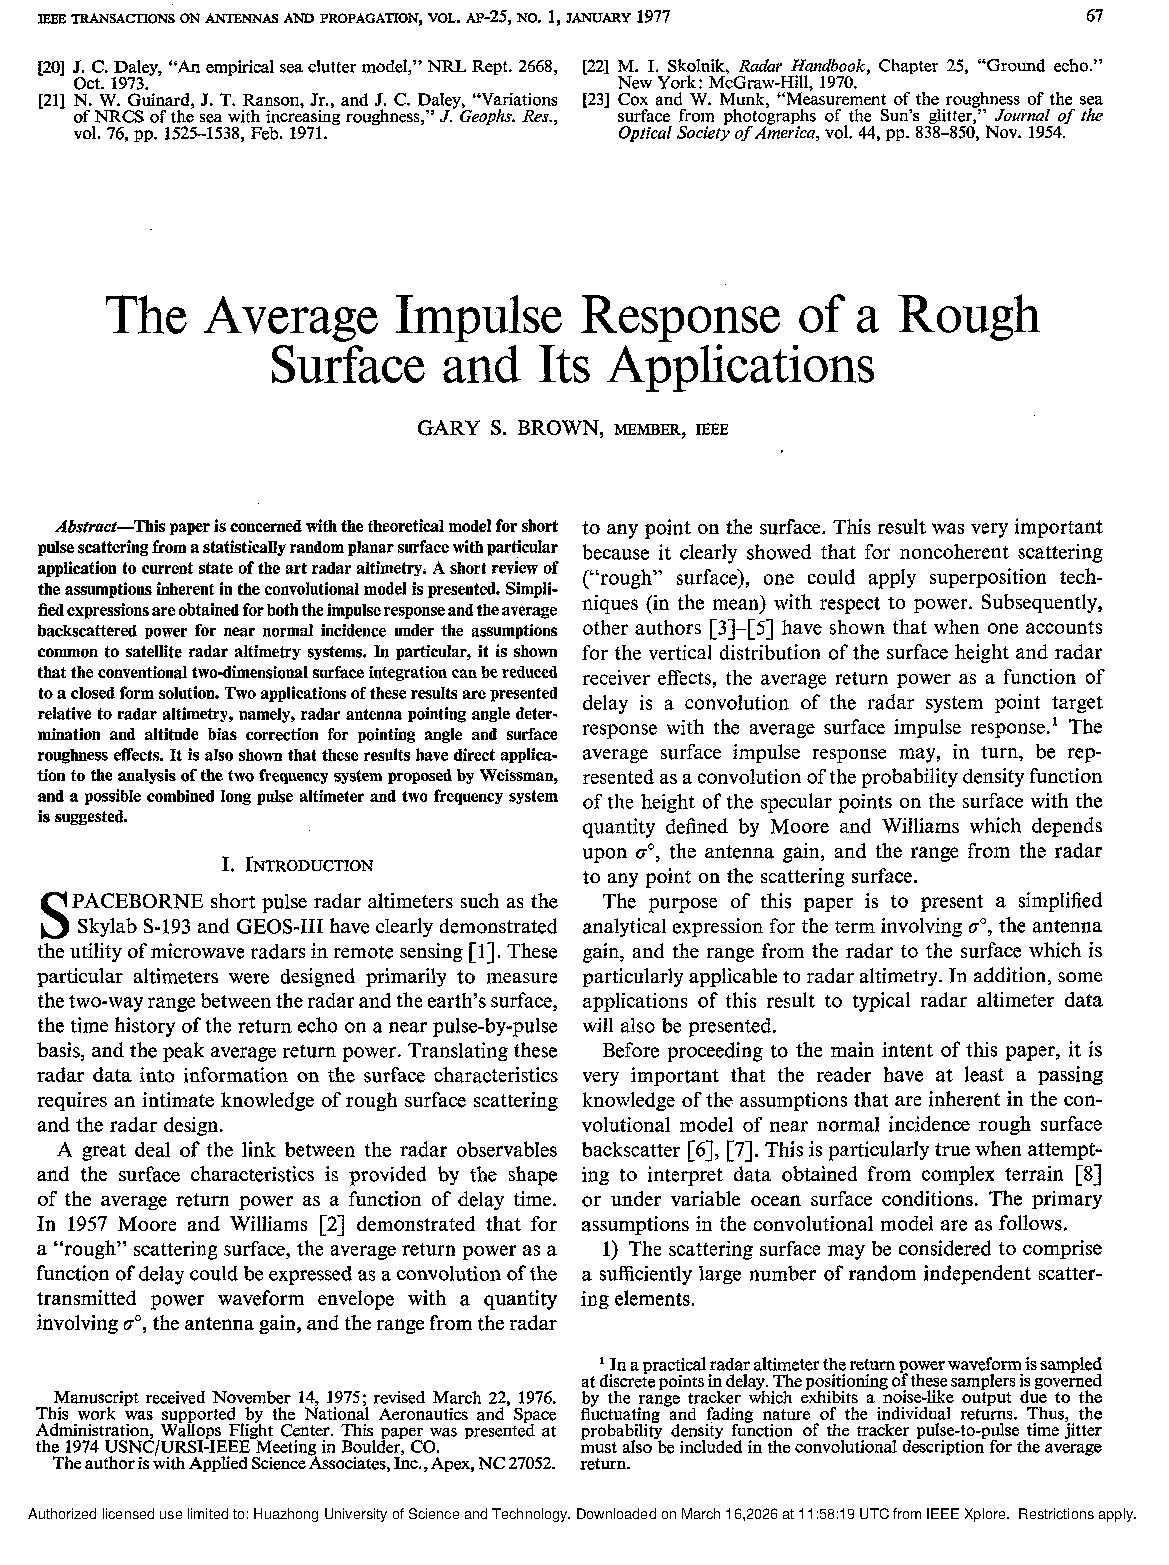
\includepdf[pages=-,pagecommand={},fitpaper=true]{The_average_impulse_response_of_a_rough_surface_and_its_applications.pdf}

\end{document}
